\pagebreak
\subsection{Aufbau des Operationsbefehls}
\label{OPbef}

\begin{figure}[h]
	\centering
	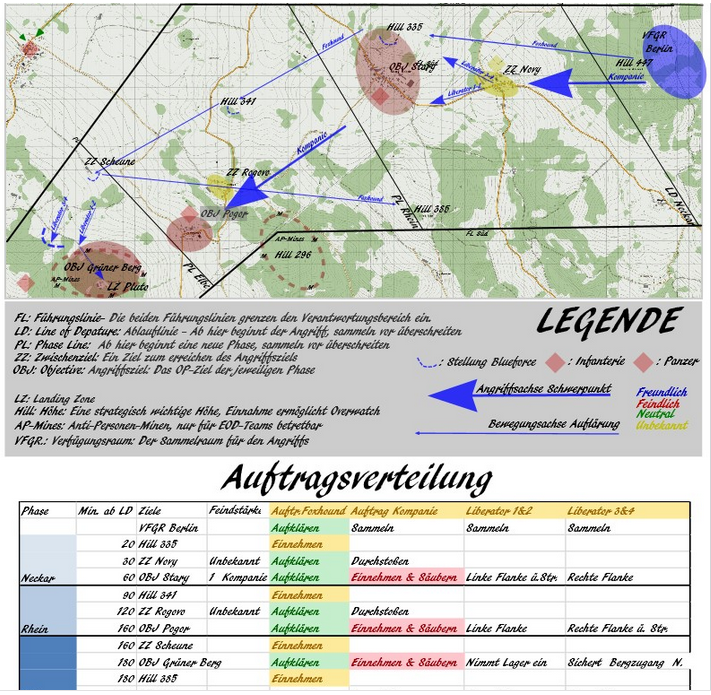
\includegraphics[width=\textwidth]{./img/fortgeschrittenes/karteUndMarkierungen/OP-Befehl}
	\caption[Ausschnitt eines Operationsbefehls]{Ausschnitt eines Operationsbefehls\footnotemark}
	\label{fig:OP-Befehl}
\end{figure}
\footnotetext{\glqq OP Der Bär erhebt sich\grqq\ -- OPL Bronko}

\subsubsection{Linien}
\begin{longtable}{P{0.2\linewidth}P{0.05\linewidth}P{0.17\linewidth}P{0.3\linewidth}P{0.13\linewidth}} 	
	\toprule
	Linien & Abk. & Bezeichnung & Anmerkung & Beispiel\\ 
	\midrule
	Führungslinie & FL & Angrenzende Himmelsrichtung & Die Führungslinien grenzen  den Verantwortungsbereich und das Operationsgebiet ein. & FL~Nord, FL~SW \\ 
	Line of Depature (Ablauflinie) & LD & Großer Fluss & Beim Überschreiten beginnt der Angriff und die Kampfhandlung & LD~Rhein, LD~Donau\\ 
	Phase Line (Kordinierungs-Führungslinie) & PL & Kleinere Flüsse & Eine OP unterteilt sich in zwei- drei räumlich und zeitlich getrennte Phasen, markiert durch die Phasenlinien & PL~Neckar, PL~Inn, PL~Isar\\ 
	Sicherungslinie & SL & Insel & Sicherungslinien, auf denen der Feind abzuwehren ist. & SL~Rügen, SL~Sylt\\ 
	\bottomrule
\end{longtable}

\subsubsection{Räume}
\begin{longtable}{P{0.2\linewidth}P{0.05\linewidth}P{0.17\linewidth}P{0.3\linewidth}P{0.13\linewidth}}
	\toprule
	Räume &	Abk. & Bezeichnung & Anmerkung & Beispiel\\ 
	\midrule
	Casualty Collection Point (Verwundeten Sammelstelle) & CCP & Verwundeten"-sammel"-stelle mit VS und Geländebeschreibung versehen & Hier werden die Verwundeten gesammelt & CCP Ruine, CCP Abdera\\
	\midrule
	Verfügungsräume	& VGR & Bundesländer, Bundesstaaten	& Sammelraum pro Phase, der als Sicher gilt. Häufig gibt es nur einen VGR vor der LD. & VGR Bayern, VGR Pfalz \\
	\midrule
	Brückenkopf & BR & Helden & Wasser"-nahe Stellung\,/\,Anlandungs"-zone im feindlichen Gebiet (Brücke, Strand, Flussseite) & BR Herakles, BR~Odin, BR~Thor \\ 
	\bottomrule
\end{longtable}

\subsubsection{Ziele und Topographie}
\begin{longtable}{P{0.2\linewidth}P{0.05\linewidth}P{0.17\linewidth}P{0.3\linewidth}P{0.13\linewidth}}
	\toprule		
	Ziele und Topographie & Abk. & Bezeichnung & Anmerkung & Beispiel \\ 
	\midrule
	Zwischenziel & ZZ &	Eingekürzter Name des Ortes oder konkrete Beschreibung des Ziels &	Zwischenziele sind optionale Ziele, je nach Schlachtverlauf zu erreichen. ZZ mit Nummer versehen! & ZZ Lager~\#1, ZZ Novograd~\#1 \\ 
	\midrule
	Objective & OBJ & Eingekürzter Name des Ortes oder konkrete Beschreibung des Ziels & Die Hauptziele der Operation & OBJ Abdera, OBJ Airport\\ 
	\midrule
	Hill (Hügel/Anhöhe) & Hill & Hügel immer mit aktueller Höhenangabe versehen. & Stratgisch wichtige Anhöhen & Hill 136\\ 
	\midrule
	Geländemarke & GM & Beschreibung, Ein, maximal zwei Wörter (Adjektiv, Subjekt) & Besondere Geländeeigenschaften werden beschrieben. &  GM~Kugelbaum, GM~tiefe Senke\\ 
	\bottomrule
\end{longtable}

\subsubsection{Zonen Luftwaffe und Logistik}
\begin{longtable}{P{0.2\linewidth}P{0.05\linewidth}P{0.17\linewidth}P{0.3\linewidth}P{0.13\linewidth}} 
	\toprule
	Zonen Luftwaffe/Logistik & Abk. & Bezeichnung & Anmerkung &	Beispiel \\ 
	\midrule
	Landezone & LZ & Nato Alphabet & Landezone, die eingerichtet werden. Dabei handelt es sich ausdrücklich um Landezonen für Helikopter. & LZ Alfa,\newline LZ Bravo\\ 
	\midrule
	Drop zone & DZ & NATO-Alphabet + \#Nummer & Dropzone, Gebiet für das Abwerfen von Mensch (FJ) und Material per Fallschirm, bzw. Slingload Drops	& DZ Alfa \#1\\ 
	\midrule
	Pick up Zone & PZ & NATO-Alphabet + \#Nummer & Zone zur Aufnahme von Mensch und Material, zum Ausfliegen oder Exfil per Boot & PZ Alfa \#1\\ 
	\midrule
	Weapon Free Zone & WFZ & Codename, Einheitenname & Zone, in der eine Einheit Feuerfrei hat, wird per Codename von OPL freigegeben. (Hier OPL, Adler Freigabe für WFZ Heureka, bestätigen sie, kommen!) & WFZ Heureka, Adler\\ 
	\midrule
	Bomben & Bomb & Codename, Einheitenname & Zone, die flächig gebombt werden soll - für Jabo, Jet-Einheiten & Bomb Hammerschlag, Condor\\ 
	\bottomrule
\end{longtable}


\subsubsection{Marsch}
\begin{longtable}{P{0.2\linewidth}P{0.05\linewidth}P{0.17\linewidth}P{0.3\linewidth}P{0.13\linewidth}} 						
	\toprule
	Marsch	& Abk. & Bezeichnung & Anmerkung & Beispiel\\ 
	\midrule
	Route, Anmarschweg & AW	& Stadt / Routenname & Route des Feindes Oder der eigene Anmarschweg	& AW Rom	\\ 
	\midrule
	Start Point (Start Punkt) & SP & Stadt / Routenname	& Startpunkt des Marsches, ab hier beginnt der Marsch & SP Rom\\ 
	\midrule
	Release Point (End Punkt) &	RP & Stadt / Routenname	& Endpunkt des Marsches, hier endet der Marsch mündet meist in ein VFGR	& RP Rom\\ 
	\midrule
	Check Point (Kontrollpunkt) & CP & Stadt / Routenname  + \#Nummer & Kontrollpunkt beim Marsch, hier wird bei passieren gemeldet, auf Befehl gehalten. & CP Rom~\#1	\\ 
	\midrule
	Passage Point (Durchlaufpunkt) & PP & Stadt / Routenname  + \#Nummer & Punkt zum Passieren, Meldung erforderlich! & PP Rom~\#1\\ 
	\midrule
	Technical Halt (Technischer Halt)) & TH & Stadt / Routenname  + \#Nummer & Technischer Halt, zum Tanken, Munitionieren, Reperatur, etc.	& TH Rom~\#1\\ 
	\bottomrule	
\end{longtable}